\hypertarget{suxe9curiser-un-site-web}{%
\section{Sécuriser un site web}\label{suxe9curiser-un-site-web}}

\begin{itemize}
\tightlist
\item
  Authentification du serveur

  \begin{itemize}
  \tightlist
  \item
    Assurer que le serveur est celui qu'il prétend être
  \end{itemize}
\item
  Intégrité des données

  \begin{itemize}
  \tightlist
  \item
    Assurer que les données reçues sont celles qui ont été envoyées
  \end{itemize}
\item
  Confidentialité des données

  \begin{itemize}
  \tightlist
  \item
    Eviter que des tiers ne puissent voir les données
  \end{itemize}
\item
  Authentification du client (optionnelle)

  \begin{itemize}
  \tightlist
  \item
    Assurer que le client est celui qu'il prétend être
  \end{itemize}
\item
  Pour un site web, ces services sont fournis par https

  \begin{itemize}
  \tightlist
  \item
    HTTPS : HTTP sécurisé par SSL/TLS, par défaut sur le port 443
  \end{itemize}
\end{itemize}

\hypertarget{secure-socket-layer-transport-layer-security}{%
\section{Secure Socket Layer --\textgreater{} Transport Layer
Security}\label{secure-socket-layer-transport-layer-security}}

\begin{itemize}
\tightlist
\item
  Conçu par Netscape (v2.0 en 1994, v3.0 en 1996)
\item
  Brevet racheté par l'IETF : TLS v1.0 en 1999 (SSL 3.1), v1.3 en 2018
\item
  Couche Application :

  \begin{itemize}
  \tightlist
  \item
    Entre les couches transport et application
  \item
    Pas besoin de modifier la pile TCP/IP
  \end{itemize}
\item
  Possibilité de sécuriser d'autres protocoles :

  \begin{itemize}
  \tightlist
  \item
    HTTP, SMTP, SIP, \ldots{}
  \end{itemize}
\item
  Services offerts :

  \begin{itemize}
  \tightlist
  \item
    Authentification serveur + intégrité données
  \item
    Confidentialité des données
  \item
    Authentification optionnelle du client
  \end{itemize}
\item
  Certificats (clé publique associée au certificat)
\end{itemize}

\hypertarget{ruxf4le-dun-certificat}{%
\section{Rôle d'un certificat}\label{ruxf4le-dun-certificat}}

\begin{itemize}
\tightlist
\item
  Garantir le lien entre une entité physique et une entité numérique :

  \begin{itemize}
  \tightlist
  \item
    Intégrité des données
  \item
    Authentification
  \item
    Confidentialité
  \end{itemize}
\item
  Document contenant une identité et une signature numérique
\item
  Utilisations courantes : https, mails
\item
  Délivré par une autorité de certification
\item
  Certificats clients
\end{itemize}

\hypertarget{autorituxe9-de-certification}{%
\section{Autorité de Certification}\label{autorituxe9-de-certification}}

\begin{itemize}
\tightlist
\item
  Tiers de confiance

  \begin{itemize}
  \tightlist
  \item
    enregistrée et certifiée par des autorités publiques ou de
    gouvernance de l'Internet
  \end{itemize}
\item
  Rôle :

  \begin{itemize}
  \tightlist
  \item
    Vérifier et garantir les informations sur l'entité
  \item
    Emettre, délivrer et révoquer les certificats
  \item
    Leur assigner une période de validité
  \item
    Maintenir la liste des certificats valides/révoqués
  \end{itemize}
\item
  Certificats auto-signés :

  \begin{itemize}
  \tightlist
  \item
    usage interne
  \item
    pas de tiers de confiance
  \end{itemize}
\end{itemize}

\hypertarget{contenu-dun-certificat-x509}{%
\section{Contenu d'un certificat
X509}\label{contenu-dun-certificat-x509}}

\begin{itemize}
\tightlist
\item
  version de X.509 (v3, depuis 1996)
\item
  numéro de série du certificat
\item
  algorithme de chiffrement utilisé pour signer le certificat
\item
  nom de l'AC émettrice
\item
  informations sur la clé publique
\item
  dates de début et fin de validité du certificat
\item
  clé publique du propriétaire du certificat
\item
  signature de l'émetteur du certificat (thumbprint)
\item
  \ldots{}
\end{itemize}

\hypertarget{composants-dune-pki1}{%
\section{\texorpdfstring{Composants d'une
\href{https://en.wikipedia.org/wiki/Public_key_infrastructure}{PKI}}{Composants d'une PKI}}\label{composants-dune-pki1}}

CA : Autorité de certification - VA : Autorité de validation - RA :
Autorité d'enregistrement
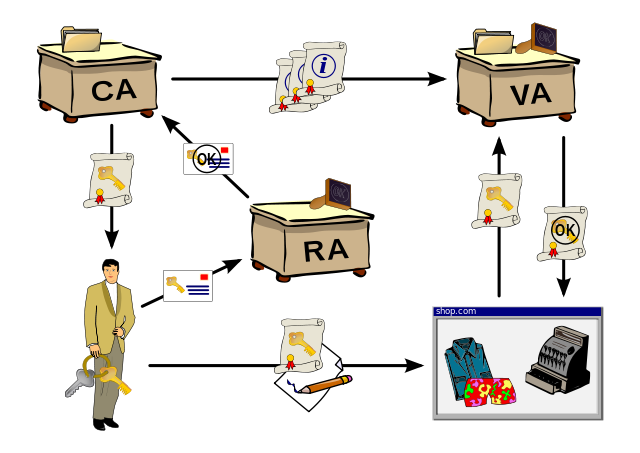
\includegraphics{src/img/Public-Key-Infrastructure.png}

\hypertarget{scuxe9nario-simplifiuxe9-de-connexion-https}{%
\section{Scénario simplifié de connexion
HTTPS}\label{scuxe9nario-simplifiuxe9-de-connexion-https}}

\begin{enumerate}
\def\labelenumi{\arabic{enumi}.}
\tightlist
\item
  Le client demande une page sécurisée
\item
  Le serveur émet sa clé publique et son certificat
\item
  Le client vérifie la validité du certificat (et qu'il correspond au
  site)
\item
  Le client utilise la clé publique pour chiffrer la clé symétrique (CS)
  utilisée ensuite
\item
  Le serveur déchiffre cette CS (avec sa clé privée) et l'utilise pour
  décoder la requête HTTPS
\item
  Le serveur répond à la requête en chiffrant avec la CS
\item
  Le navigateur décode la réponse avec la CS
\end{enumerate}

\begin{itemize}
\tightlist
\item
  En
  \href{https://tiptopsecurity.com/how-does-https-work-rsa-encryption-explained/}{images},
  \href{http://software-engineer-tips-and-tricks.blogspot.ch/2012/08/ssl-in-pictures.html?view=sidebar}{ou
  ici} ou en
  \href{https://www.youtube.com/embed/iQsKdtjwtYI?rel=0}{slides}
\item
  2-5 en TCP
\end{itemize}

\hypertarget{duxe9ploiement}{%
\section{Déploiement}\label{duxe9ploiement}}

\begin{itemize}
\tightlist
\item
  Installer OpenSSL
\item
  (Créer son autorité de certification si autosigné)
\item
  Obtenir le certificat et la clé privée du serveur
\item
  Configurer httpd. Pour Apache :

  \begin{itemize}
  \tightlist
  \item
    virtual host (port 443), ssl.conf, (ports.conf)
  \end{itemize}
\item
  Création de l'arborescence sécurisée
\item
  Démarrage serveur
\item
  OU BIEN utiliser \href{https://letsencrypt.org/}{Let's encrypt}
\item
  OU BIEN utiliser un serveur pré-configuré comme
  \href{https://caddyserver.com/}{Caddy}
\end{itemize}

\hypertarget{https-aujourdhui}{%
\section{HTTPS Aujourd'hui}\label{https-aujourdhui}}

\begin{itemize}
\tightlist
\item
  Il n'y a plus de bonne raison d'utiliser HTTP
\item
  TLS toujours utilisé avec HTTP2 et HTTP3
\item
  HTTP2 et 3 minimisent et accélèrent les échanges
\item
  Certificats gratuits
\item
  Mise en place simplifiée
\end{itemize}

\hypertarget{ressources}{%
\section{Ressources}\label{ressources}}

\begin{itemize}
\tightlist
\item
  \href{https://wiki.alphanet.ch/Ateliers/PresentationSecurityParty}{Security
  Party 23.10.2009}
\item
  \href{http://www.sebsauvage.net/comprendre/ssl/}{SebSauvage}
\item
  HTTPS en détails :

  \begin{itemize}
  \tightlist
  \item
    Diagramme de séquence
    \href{https://www.eventhelix.com/networking/SSL.pdf}{HTTPS}
  \item
    Diagramme de séquence
    \href{https://www.eventhelix.com/networking/ssl-tls/https-ssl-tls-session-for-spdy.pdf}{SPDY}
  \item
    \href{https://security.stackexchange.com/questions/20803/how-does-ssl-tls-work/20847\#20847}{SSL}
    en détails
  \end{itemize}
\item
  Durée de vie de la
  \href{https://security.stackexchange.com/questions/55454/how-long-does-an-https-symmetric-key-last}{Clé
  Symétrique}
\item
  \href{https://www.win.tue.nl/hashclash/rogue-ca/}{Faux Certificat}
\item
  Autorités de certification :

  \begin{itemize}
  \tightlist
  \item
    \href{https://letsencrypt.org/}{Let's Encrypt}
  \item
    \href{http://www.cacert.org/}{CA Cert}
  \item
    \href{https://www.sslforfree.com/}{SSLforFree}
  \end{itemize}
\item
  Différences TLS / SSH :
  \href{http://www.snailbook.com/faq/ssl.auto.html}{Snailbook},
  \href{http://security.stackexchange.com/questions/1599/what-is-the-difference-between-ssl-vs-ssh-which-is-more-secure}{StackExchange}
\end{itemize}

\hypertarget{sources}{%
\section{Sources}\label{sources}}
